\documentclass[sigconf]{acmart}
\usepackage{graphicx}
\fancyhf{} % Remove fancy page headers 
\fancyhead[C]{Brian Vannah's CS460 HW5} 
\fancyfoot[C]{\thepage}

\setcopyright{none} % No copyright notice required for submissions
\acmConference[Brian Vannah's Submission for Homework 5]{CS460: Intro Computer and Network Security}{Due 20 December 2018}{Amherst, Massachusetts}
\acmYear{2018}

\settopmatter{printacmref=false, printccs=true, printfolios=true} % We want page numbers on submissions


\begin{document}
\title{Applications of Steganography: Who Uses it?}
\author{Brian Vannah}
\begin{abstract}
Anyone with a laptop and some basic coding skills can use steganography. But, who actually uses it? Perhaps more importantly, who should? This paper will attempt to answer those questions while giving a few interesting examples of usage. 
\end{abstract}

 \begin{CCSXML}
<ccs2012>
<concept>
<concept_id>10010405.10010462</concept_id>
<concept_desc>Applied computing~Computer forensics</concept_desc>
<concept_significance>100</concept_significance>
</concept>
</ccs2012>
\end{CCSXML}

\ccsdesc[100]{Applied computing~Computer forensics}
% -- end of section to replace with generated code

\keywords{steganography, covert communication, printers, espionage} 

\maketitle



\section{Introduction}
	Covert communication can take many forms. One interesting form is steganography, which is a way of hiding information in digital media such as pictures or sound files.

	Covert forms of communication could have a wide variety of uses, but those uses are secret by design. When people use steganography, they generally don't want other people to know about it. If the information about how people use steganography to send hidden messages was public it would defeat the purpose of using it. If someone knows the covert channel that you are using, it is easy for them to intercept your messages. 

	Due to the nature of secrecy, there are speculations that various organizations are using covert communication such as steganography to send secret information. Some people think that the FBI and Al-Queda use steganography to post hidden messages on eBay, Reddit, and various pornographic websites, and this theory appeared in U.S. news outlets~\cite{cnn}. But, who actually uses steganography? Some researchers say "basically nobody."

	A 2001 analysis of over 2 million images from eBay revealed no steganographic content~\cite{provos}. The test for steganography in that research analysis paper involved looking for statistical anomalies within the image data. Images with hidden data were expected to have more randomness than those without. The researchers developed several statistical algorithms for detecting hidden content in images. On the 2 million eBay images, the algorithms found about 17,000 possible images with secret hidden data. With those images, the researchers then did a dictionary/brute force attack to try to guess the passwords used to encode the data within the image. They found no hidden messages of any kind. So, the researchers concluded that it was highly likely that there was no steganographic content on eBay. It's true that it's possible that the researchers just couldn't guess the password. However, there are usually at least a small proportion of passwords that are weak and easily guessed, so the researchers contend that if steganography was being used commonly, they would have seen at least some evidence of it. It's also true that it's possible that people may have used steganographic methods beyond the detection of the researchers. However, if there were a lot of people using steganography, at least some of them would have used methods simple enough to be detected by researchers. Therefore, the researchers concluded that it was highly likely that no one was using eBay to post hidden messages in images.


\section{Printers}  
	In the 1980's, computer printers were becoming more common in average households. This made it much easier for people to copy documents. One consequence of this is that it became easier to counterfeit or illegally reproduce documents. To track such documents, Xerox began encoding data into printed pages which went unnoticed by the human eye. Each page printed has a matrix where small yellow dots could be printed, which indicate bits of data about the printed page (see Figure 1). 
\begin{figure}[h]
\caption{Barely-noticeable yellow dots indicating data on a printed page ~\cite{wikiuser}.}
\centering
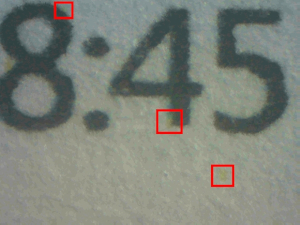
\includegraphics[scale=1.06]{fig1}
\end{figure}
	Each yellow dot (or lack of a dot) represents one bit of data about the printing. The data encoded most often includes the printer's serial number and the time of printing (see Figure 2). 
\begin{figure}[h]
\caption{How some of the yellow dots are decoded ~\cite{EFF}.}
\centering
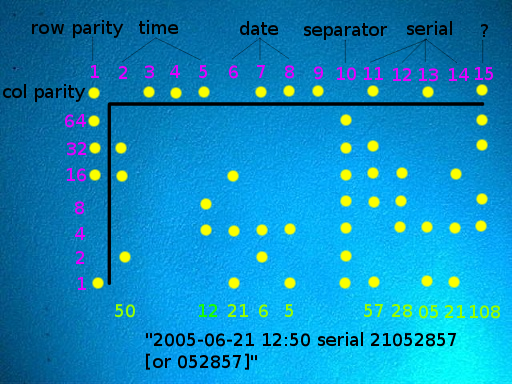
\includegraphics[scale=.47]{fig2}
\end{figure}
	This practice was later adopted by most (if not all) commercial printing companies, including HP, Dell, Brother, and Canon. The Electronic Frontier Foundation ~\cite{EFF} claims that all commercial printers print some kind of forensic tracking information on documents, sometimes without the knowledge of costumers. Some encoding types remain unknown to the public, so many people do not know how their documents are tracked. Writing the serial number on documents can relate a document to the printer on which it was created, which is very useful for criminal investigations. The printing industry has been extraordinarily helpful to law enforcement, especially the U.S. Secret Service, which deals with many of the counterfeiting cases~\cite{pcworld}. 

	However, the tracking of serial numbers and other data is not good for everyone. Whistleblowers and others who seek to print anonymously cannot do so. There is software to cover up the tracking dots and the places where they might appear, therefore making the encoded data impossible to read. An example of such software is DEDA~\cite{deda}, which recognizes yellow dot patterns and removes the cells in which they might appear. DEDA fills in all of the tracking dot matrix with the regular white color, so when the information is decoded, every bit is 0, making all of the data nonsensical. This prevents tracking, because all of the pages with the false data would show up as being created at time 0 by printer with serial number 0. However, this software doesn't always work because a lot of encoding mechanisms are unknown by the software developers. Some printer manufacturers are reluctant to tell the public what data is printed, or how it is printed. This leaves the decoding up to the costumers, and some printer encodings remain a mystery.

	People don't like that their data is being shared, even on a small scale. The mysterious, unknown aspect of how printer steganography is used only heigtens the paranoia around the subject. A demonstration of the paranoia and outrage is seeingyellow.com, a website that posts information about the tracking dots as well as instructions on how to call your printer manufacturer to complain. They claim that 48966 people have followed their instructions to call printer manufacturers to try to stop the data encoding. The website also claims that one anonymous person called to complain about the printer data encoding and was questioned by Secret Service agents at their house a few days later.

	Steganography and covert channels in general are designed to be secret and mysterious. Perhaps it is only natural that printer manufacturers using steganography would not want to release information about how it is used. If everyone knew how the steganography worked and could be decoded, then anyone could find and decode the dots. Then, the printers might as well just print the data in readable text. Perhaps manufacturers use steganography because they want the information to be available to the manufacturers and law enforcement, but not the general public (for privacy reasons). Law enforcement can ask/subpoena the manufacturers for the decoding algorithms, and keep those algorithms a secret. That way, a random person who gets your publication does not have your serial number and other information, but the police can get it if they need it. This approach is flawed because security through obscurity hardly ever works (Kerckhoff's Principle). Eventually, someone will figure out the decoding algorithm and then an unintend user will be able to get the information.

	Perhaps a better approach to implementing printer tracking would be to use some form of cryptography to encrypt the data using the manufacturer's public key. That encrypted data could be printed in readable text or as a QR code in the corner of the page. There would be no need for a certificate authority to verify the public key, because the public key of the manufacturers could be built into the machine when the printer is created. Therefore, this approach would not be vulnerable to rogue certificate authorities or fake-key attacks. A possible downside to this approach is that each document printed from the same printer would have the same serial number. If the serial number is encrypted the same way each time, then the same bytes would appear in the ciphertext, which would leak information about the serial number. Furthermore, if two pages had the same "serial number" ciphertext, then an adversary would know that they were made by the same printer. Similarly, if the "time" ciphertext was the same, an adversary would know that they were printed at the same time. Therefore, it would be worthwhile to choose a cryptographic algorithm that adds salt or random data to the serial number and time before they are encrypted.

	Using this approach, printer manufacturers could still provide the private key or decrypted plaintext to law enforcement, allowing them to track documents when needed. Altogether, the cryptographic approach would allow printing manufacturers to maintain the same usefulness for law enforcement while eliminating the risk that unauthorized people would be able to decode their secret data. Furthermore, the cryptographic approach would make it more feasible for manufacturers to publish the details of how customers' data is being printed. This would ease the minds of customers who hate that their data is being used in unknown ways, like those people on seeingyellow.com. Manufacturers could even keep the same yellow dot printing instead of switching to printing the data as readable text or a QR code. All they would have to do is add on the additional layer of security in cryptography, which would obviously make the data more secure and let manufacturers publish the information about how users' data is printed. Moving away from the steganography approach of "security through obscurity" would have a lot of benefits for the printing industry.

\section{Espionage}

	Anna Kushchyenko was a Russian spy. She was the typical spy like those in the movies, pretending to be an alternate identity. In 2001, she was spying or travelling in London, where she met Alex Chapman at a dance party. Alex Chapman was a British citizen, and did not know that Kushyenko was a spy. The two got married, and Anna Kushchyenko became Anna Chapman and gained British citizenship. A few years later, she used her British citizenship to get American residence, moving to New York in 2009. She was posing as an American citizen and CEO of PropertyFinder LLC, attempting to use her status to make contacts with important Americans and gaining intelligence ~\cite{dt}.
	
	To communicate with her employer and contacts in Russia, Chapman used steganography. Her employer, the Moscow Center in Russia, developed their own steganography software instead of using commercially available software, to increase the obscurity. Anna Chapman used the software to post images on various websites, which contained the secret messages she was sending to Russia. The software also used cryptography at the same time, to increase security by making the user enter a 27-character password. However, when the time came and the FBI took her hard drive in 2010, they were able to find, decode, and decrypt the messages within the images. Using her browser website history, investigators were able to see where she was posting the images. They could then download and analyze the images, using the steganography software on her computer and the 27-character password (which was written on a notepad in her home). Altogether, the FBI was able to read over 100 messages hidden in different images ~\cite{doc}.

	Using picture steganography led to the decoding of the messages. Picture steganography is outdated, because it's hard to hide a lot of data in a single picture. So, users have to post lots of pictures, and each picture posted leaves a trail, whether it's a source and destination of an email, or browser history to the image posting website. A better approach would have been to use network steganography, which puts data into network traffic similar to how picture steganography puts data into pictures. Network steganography can use a variety of channels (see Figure 3), such as timing, handshake protocols, intentional packet errors and intentionally fragmented messages~\cite{net}. 
\begin{figure}[h]
\caption{Examples of network steganography channels on each layer of the network model ~\cite{net}}
\centering
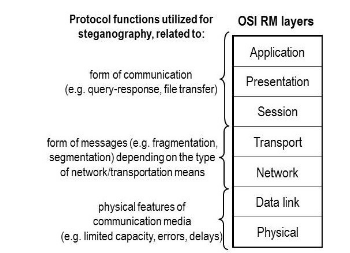
\includegraphics[scale=2.3]{fig3}
\end{figure}
	With such a wide variety of methods to use, network steganography can be much more obscure than picture steganography, allowing for more secrecy. Since obscurity is essentially the goal of steganography, network steganography would have been a better approach for Anna Chapman and the Russians. Then, maybe her messages would not have been decoded.


\section{Conclusion}
	The eBay research ~\cite{provos} was done in 2001, which was when notably fewer people had access to and knowledge about computers. In 2018, everyone has smartphones and lots of people have laptops and coding knowledge. Basic encoding schemes could be simple enough for lots of computer users to understand, so steganography could be widely used. Picture steganography is interesting and easy to get started with, and there are more advanced forms such as network steganography that provide more secrecy. With all of this in mind, it would be very surprising if there were not lots of people using steganography in 2018, even if researchers in 2001 concluded that no one was using it.

	Who should not use stegaonography? As discussed earlier, printer manufacturers could benefit greatly by moving away from steganography. In general, companies or other organizations that do a lot of communication with the public should not use steganography. Since the steganography medium (in this case, the printed pages) can be viewed by a lot of people, there is more of a risk that someone will figure out how to decode or expose the data hidden in the medium. The low level of security through obscurity that steganography provides is not worth the drawbacks of publicity and paranoia. 

	Who should use steganography? People who rely on secrecy, and do communication that is less likely to be seen. People like Anna Chapman, who may communicate over secret channels with the Russians. Her messages were only read by a few people, because she wasn't printing them out in billions of printers. Fewer people were looking at Chapman's posted images than the printed pages, so the algorithm was less likely to be discovered. However, her steganography failed in the end because of her use of basic picture steganography. She should instead have used more complicated forms such as network steganography. 
	
	Different reasons for communicating may lead to different approaches to covert communication. Printer manufacturers may have different needs and desires than secret agents. Hobbyists, spies, and researchers may enjoy hiding their communications however they want. But, in general, more obscure and hidden forms of steganography will provide more secrecy. 


\appendix
%%\begin{acks}
%%\end{acks}
 % TODO: replace with your brilliant paper!

\bibliographystyle{ACM-Reference-Format}
\bibliography{ccs-sample}

\end{document}
